% Pilot run of the study configuration (DeepSeek-V4-Flash).
% Numbers come from aaai27/figures/data/pilot_*.csv, extracted from the run
% directory with aaai27/figures/scripts/extract_pilot_run.py; the figure is
% rebuilt with aaai27/figures/scripts/make_figures.py.
\providecommand{\shrlm}{\textsc{SH-RLM}\xspace}

\section{Pilot Run of the Study Configuration}
\label{sec:pilot}

Before the full study, we ran the optimization loop at reduced size on OOLONG-Pairs with the study backbone,
DeepSeek-V4-Flash (temperature 0, \$0.19/\$0.51 per million input/output
tokens). It starts from \hzero and uses the blended 8K/16K/32K strata, the F1
gate of Equation~\ref{eq:promotion-main} with frozen margins
$\tau_\ell=.144/.144/.244$ and $\tau_{\mathrm{imp}}{=}0.02$, the cost band
$[0.5,3]\times$, $m{=}2$, $v{=}3$, $k{=}4$, and one screening task per stratum
with one attempt. Mining and validation each use 4 tasks per stratum, half the
study size, so each validation subject is 36 runs. The run is a single
trajectory and was stopped after four rounds. Its held-out tasks are validation
tasks, not test tasks, so it measures the loop, not the final harness.
\Cref{fig:pilot} summarizes every gate decision.

\begin{figure*}[t]
\centering
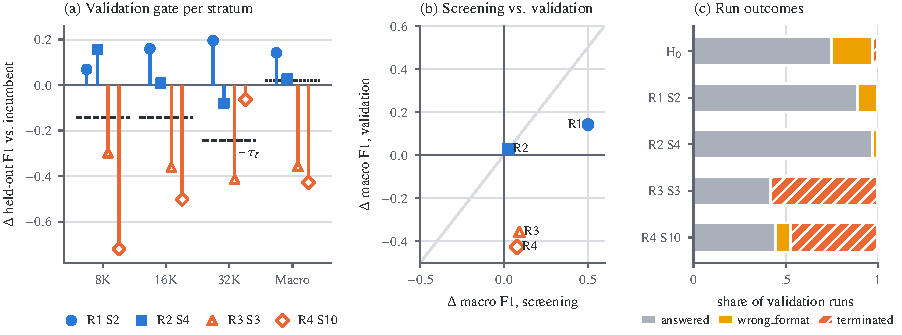
\includegraphics[width=\textwidth]{aaai27/figures/fig_pilot_gate.pdf}
\caption{Pilot run (DeepSeek-V4-Flash, OOLONG-Pairs, 12 validation tasks
$\times$ 3 attempts per subject). Filled blue markers are promoted
candidates and hollow orange markers are rejected ones; R$t$~S$j$ is the round
and edited surface. (a)~Held-out F1 change against the round's incumbent per
stratum and macro-averaged. Dashed lines are the veto margins $-\tau_\ell$; the
dotted line is $\tau_{\mathrm{imp}}$. (b)~Macro-F1 change in screening (3 tasks
$\times$ 1 attempt) against full validation; the grey line is $y{=}x$.
(c)~Outcome of the 36 validation runs: a scored answer, a malformed answer
(\texttt{wrong\_format}, F1 $=0$), or termination by the 3,600\,s cap (F1
$=0$). Incumbent rows after round 1 reuse the previous candidate's runs and
are omitted.}
\label{fig:pilot}
\end{figure*}

\paragraph{Two promotions.}
Round 1 mined mostly \texttt{mixed\_set\_error} failures and promoted an
\sid{S2} edit that restates in the decomposition instruction that the final
output is a set of user-ID pairs. Held-out macro F1 rose from .565 to .707
($+.141$), with gains at every stratum (\cref{fig:pilot}a). Most of the gain
came from fewer malformed answers: \texttt{wrong\_format} runs fell from 8 to
4 of 36 (\cref{fig:pilot}c), while F1 on runs that returned a scored answer rose
only from .754 to .795. Mean sub-calls per run fell from 262 to 160 at the same
cost per run. Round 2 promoted an \sid{S4} verification edit that makes the
root reclassify questions it finds misclassified. Exact passes rose from 4 to 7
of 36 and 8K F1 rose by $+.157$, but 16K moved by only $+.008$ and 32K fell by
$.081$. The 32K drop sits well inside its margin of $.244$, and the macro gain
of $+.028$ clears $\tau_{\mathrm{imp}}$ by $.008$, so the gate promoted a
harness that is worse at the longest optimization length. Cost per run rose
$1.41\times$.

\paragraph{Screening does not predict validation.}
Rounds 3 and 4 validated an \sid{S3} instruction edit and an \sid{S10} skill,
both aimed at round~3's mined classification failures: a batch loop that
silently drops questions, and spot-checks that miss misclassified ones. Both
won screening against the incumbent, by $+.091$ and $+.078$ macro F1, and both
then lost $.358$ and $.428$ in validation (\cref{fig:pilot}b). Screening with
one attempt per stratum is dominated by single runs: the same round-1
incumbent scored 0 on its only 16K screening run, and the round-2 incumbent
scored .913 in screening against .707 in validation. Across the four validated
candidates the screening sign matched the validation sign twice. Screening
therefore orders candidates with little information, and only full validation
protected the incumbent here.

\paragraph{How the rejected candidates failed.}
Both rejected candidates stopped delegating. Mean sub-calls fell from 116 to
12 and 13 per run, and 21 and 17 of the 36 runs hit the 3,600\,s cap
(\cref{fig:pilot}c), each scoring 0. When the \sid{S3} candidate did answer,
its F1 was .905 against the incumbent's .756, so the edit improved the
classification it targeted but moved that work into slow root-level loops.
The gate rejected both on every stratum except the \sid{S10} candidate's 32K
stratum, and also because their cost per run fell below $0.5\times$ the
incumbent's. The loop's refinement step did not fire for \sid{S3}, because its
trigger is a higher \texttt{wrong\_format} rate and the failures were
terminations. A refinement trigger keyed to resource terminations would have
targeted this failure.

\paragraph{Mining and validation disagree on difficulty.}
On the held-in mining tasks the incumbent's macro F1 was .884, .904, and .891
in rounds 1--3, while its held-out validation F1 was .565, .707, and .735.
Mining saw a malformed answer in 1 of 24 \hzero runs, against 8 of 36 in
validation. The round-1 gain came mostly from fixing that failure, so it was
measured on a failure that mining had barely seen. With 4 tasks per stratum,
which predicates fall in each split changes what the loop can learn.

\paragraph{Cost.}
The four rounds cost at least \$39.1 in model calls (some stage totals are
lower bounds). Validation took \$25.6 (65\%), screening \$7.2, mining \$6.2,
and attribution and proposal together \$0.16. Proposing edits is cheap;
deciding whether to keep them is not.
